% (find-LATEX "2021-2-C2-infs-e-sups.tex")
% (defun c () (interactive) (find-LATEXsh "lualatex -record 2021-2-C2-infs-e-sups.tex" :end))
% (defun C () (interactive) (find-LATEXsh "lualatex 2021-2-C2-infs-e-sups.tex" "Success!!!"))
% (defun D () (interactive) (find-pdf-page      "~/LATEX/2021-2-C2-infs-e-sups.pdf"))
% (defun d () (interactive) (find-pdftools-page "~/LATEX/2021-2-C2-infs-e-sups.pdf"))
% (defun e () (interactive) (find-LATEX "2021-2-C2-infs-e-sups.tex"))
% (defun o () (interactive) (find-LATEX "2021-2-C2-infs-e-sups.tex"))
% (defun u () (interactive) (find-latex-upload-links "2021-2-C2-infs-e-sups"))
% (defun v () (interactive) (find-2a '(e) '(d)))
% (defun d0 () (interactive) (find-ebuffer "2021-2-C2-infs-e-sups.pdf"))
% (defun cv () (interactive) (C) (ee-kill-this-buffer) (v) (g))
%          (code-eec-LATEX "2021-2-C2-infs-e-sups")
% (find-pdf-page   "~/LATEX/2021-2-C2-infs-e-sups.pdf")
% (find-sh0 "cp -v  ~/LATEX/2021-2-C2-infs-e-sups.pdf /tmp/")
% (find-sh0 "cp -v  ~/LATEX/2021-2-C2-infs-e-sups.pdf /tmp/pen/")
%     (find-xournalpp "/tmp/2021-2-C2-infs-e-sups.pdf")
%   file:///home/edrx/LATEX/2021-2-C2-infs-e-sups.pdf
%               file:///tmp/2021-2-C2-infs-e-sups.pdf
%           file:///tmp/pen/2021-2-C2-infs-e-sups.pdf
% http://angg.twu.net/LATEX/2021-2-C2-infs-e-sups.pdf
% (find-LATEX "2019.mk")
% (find-CN-aula-links "2021-2-C2-infs-e-sups" "2" "c2m212is" "c2is")

% «.defs»		(to "defs")
% «.title»		(to "title")
% «.introducao»		(to "introducao")
% «.set-compr»		(to "set-compr")
% «.set-compr-2»	(to "set-compr-2")
% «.set-compr-traducao»	(to "set-compr-traducao")
% «.fa-e-ex-traducao»	(to "fa-e-ex-traducao")
% «.programa-1»		(to "programa-1")
% «.programa-2»		(to "programa-2")
% «.eixo-y»		(to "eixo-y")
% «.exercicio-1»	(to "exercicio-1")
% «.uma-figura»		(to "uma-figura")
% «.exercicios-23»	(to "exercicios-23")
% «.exercicios-4567»	(to "exercicios-4567")
% «.exercicio-10»	(to "exercicio-10")
%
% «.djvuize»	(to "djvuize")



% <videos>
% Video (not yet):
% (find-ssr-links     "c2m212is" "2021-2-C2-infs-e-sups" "{naoexiste}")
% (code-eevvideo      "c2m212is" "2021-2-C2-infs-e-sups")
% (code-eevlinksvideo "c2m212is" "2021-2-C2-infs-e-sups")
% (find-c2m212isvideo "0:00")

\documentclass[oneside,12pt]{article}
\usepackage[colorlinks,citecolor=DarkRed,urlcolor=DarkRed]{hyperref} % (find-es "tex" "hyperref")
\usepackage{amsmath}
\usepackage{amsfonts}
\usepackage{amssymb}
\usepackage{pict2e}
\usepackage[x11names,svgnames]{xcolor} % (find-es "tex" "xcolor")
\usepackage{colorweb}                  % (find-es "tex" "colorweb")
%\usepackage{tikz}
%
% (find-dn6 "preamble6.lua" "preamble0")
%\usepackage{proof}   % For derivation trees ("%:" lines)
%\input diagxy        % For 2D diagrams ("%D" lines)
%\xyoption{curve}     % For the ".curve=" feature in 2D diagrams
%
\usepackage{edrx21}               % (find-LATEX "edrx21.sty")
\input edrxaccents.tex            % (find-LATEX "edrxaccents.tex")
\input edrx21chars.tex            % (find-LATEX "edrx21chars.tex")
\input edrxheadfoot.tex           % (find-LATEX "edrxheadfoot.tex")
\input edrxgac2.tex               % (find-LATEX "edrxgac2.tex")
%
%\usepackage[backend=biber,
%   style=alphabetic]{biblatex}            % (find-es "tex" "biber")
%\addbibresource{catsem-slides.bib}        % (find-LATEX "catsem-slides.bib")
%
% (find-es "tex" "geometry")
\usepackage[a6paper, landscape,
            top=1.5cm, bottom=.25cm, left=1cm, right=1cm, includefoot
           ]{geometry}
%
\begin{document}

\catcode`\^^J=10
\directlua{dofile "dednat6load.lua"}  % (find-LATEX "dednat6load.lua")
\directlua{dofile "2021verbatim.lua"} % (find-LATEX "2021verbatim.lua")
\directlua{dofile "2021pict2e.lua"}   % (find-LATEX "2021pict2e.lua")
%L Pict2e.__index.suffix = "%"
\pu
\def\pictgridstyle{\color{GrayPale}\linethickness{0.3pt}}
\def\pictaxesstyle{\linethickness{0.5pt}}




% «defs»  (to ".defs")
% (find-LATEX "edrx21defs.tex" "colors")
% (find-LATEX "edrx21.sty")

\def\u#1{\par{\footnotesize \url{#1}}}

\def\drafturl{http://angg.twu.net/LATEX/2021-2-C2.pdf}
\def\drafturl{http://angg.twu.net/2021.2-C2.html}
\def\draftfooter{\tiny \href{\drafturl}{\jobname{}} \ColorBrown{\shorttoday{} \hours}}



%  _____ _ _   _                               
% |_   _(_) |_| | ___   _ __   __ _  __ _  ___ 
%   | | | | __| |/ _ \ | '_ \ / _` |/ _` |/ _ \
%   | | | | |_| |  __/ | |_) | (_| | (_| |  __/
%   |_| |_|\__|_|\___| | .__/ \__,_|\__, |\___|
%                      |_|          |___/      
%
% «title»  (to ".title")
% (c2m212isp 1 "title")
% (c2m212isa   "title")

\thispagestyle{empty}

\begin{center}

\vspace*{1.2cm}

{\bf \Large Cálculo 2 - 2021.2}

\bsk

Aula 17: infs e sups

\bsk

Eduardo Ochs - RCN/PURO/UFF

\url{http://angg.twu.net/2021.2-C2.html}

\end{center}

\newpage

%  ___       _                 _                       
% |_ _|_ __ | |_ _ __ ___   __| |_   _  ___ __ _  ___  
%  | || '_ \| __| '__/ _ \ / _` | | | |/ __/ _` |/ _ \ 
%  | || | | | |_| | | (_) | (_| | |_| | (_| (_| | (_) |
% |___|_| |_|\__|_|  \___/ \__,_|\__,_|\___\__,_|\___/ 
%                                                      
% «introducao»  (to ".introducao")
% (c2m212isp 2 "introducao")
% (c2m212isa   "introducao")

{\bf Introdução}


\scalebox{0.6}{\def\colwidth{9cm}\firstcol{

    Infs e sups são um dos assuntos secundários de Cálculo 2 que vão
    ser mais úteis para as matérias seguintes. Infs e sups vão
    aparecer {\sl explicitamente} nas próximas matérias muito poucas
    vezes, mas pra aprender infs e sups a gente vai ter que aprender
    as quatro coisas absurdamente úteis abaixo. Vamos ter que:

    \begin{itemize}

    \item aprender um certa linguagem formal pra descrever conjuntos
      -- chamada de ``set comprehensions'' em inglês. Vou adaptar o
      material daqui:

      {\footnotesize

        % (mpgp 8 "comprehension")
        % (mpga   "comprehension")
        % http://angg.twu.net/LATEX/material-para-GA.pdf#page=8
        \url{http://angg.twu.net/LATEX/material-para-GA.pdf\#page=8}

      }

    \item aprender a visualizar certas operações -- usando ``tipos'' e
      os truques com bolinhas brancas e pretas que nós começamos a ver
      nas páginas 11 até 20 deste PDF daqui:

      {\footnotesize

        % (c2m212somas2p 11 "tipos")
        % (c2m212somas2a    "tipos")
        % http://angg.twu.net/LATEX/2021-2-C2-somas-2.pdf
        \url{http://angg.twu.net/LATEX/2021-2-C2-somas-2.pdf}

      }

    \end{itemize}


}\anothercol{


  \begin{itemize}

  \item aprender a lidar com contas que à primeira vista exigiriam um
    número infinito de operações e portanto um número infinito de
    páginas. Lembre que \ColorRed{Cálculo 2 não é Cálculo 1} -- em
    Cálculo 1 a gente aprende a fazer contas que chegam direto na
    solução, mas Cálculo 2 é baseado em \ColorRed{chutar e testar}, e
    nesta parte da matéria nós vamos usar o ``chutar e testar'' pra
    reconhecer padrões... aí ao invés da gente fazer as contas pra
    infinitos casos um de cada vez a gente vai começar fazendo elas
    pra, digamos, 5 casos, e ver se com esses 5 casos a gente consegue
    entender visualmente o que as nossas contas ``querem dizer''.

  \item aprender a fazer argumentos informais, com desenhos e explicaões
    em português, que todo mundo entenda. Releia este PDF aqui:

    {\footnotesize

      % (c2m212somas24p 1 "title")
      % (c2m212somas24a   "title")
      \url{http://angg.twu.net/LATEX/2021-2-C2-somas-2-4.pdf}

    }

  \end{itemize}


}}


\newpage

% «set-compr»  (to ".set-compr")
% (c2m212isp 3 "set-compr")
% (c2m212isa   "set-compr")

{\bf Set comprehensions}

Quando eu dava Geometria Analítica e as aulas eram presenciais eu
começava o curso com uns exercícios de ``set comprehensions'' -- os
das páginas 8 a 12 deste PDF:

% (mpgp 8 "comprehension")
% (mpga   "comprehension")

\ssk

{\footnotesize

  % (mpgp 8 "comprehension")
  % (mpga   "comprehension")
  % http://angg.twu.net/LATEX/material-para-GA.pdf#page=8
  \url{http://angg.twu.net/LATEX/material-para-GA.pdf\#page=8}

}

\ssk

Eu dividia a turma em grupos de 5 pessoas e dizia: ``tentem entender
isso aqui a partir dos exemplos e das poucas explicações em português.
Vocês {\sl provavelmente} vão conseguir entender quase tudo só
discutindo entre vocês, tentando fazer os exercícios -- inclusive os
que têm umas pegadinhas difíceis -- e comparando os resultados de
vocês com os dos colegas, mas qualquer coisa me chamem''... e eu
ficava circulando pela sala ajudando os grupos. Isso funcionava super
bem, e geralmente em uma aula só de duas horas quase todo mundo
conseguia fazer os exercícios.


\newpage

% «set-compr-2»  (to ".set-compr-2")
% (c2m212isp 4 "set-compr-2")
% (c2m212isa   "set-compr-2")

{\bf Set comprehensions (2)}

Como 1) as turmas estão meio desanimadas, com pouca gente participando
das discussões e 2) todo mundo já fez Prog 1, eu vou usar um método
diferente. Eu vou complementar a parte de ``set compreensions'' do
``Material para GA'' mostrando como traduzir as notações dele pra um
pseudocódigo bem parecido com {\tt C}, e a gente vai seguir direto
pros exercícios com mais cara de Cálculo 2 e de infs e sups.

\msk

Basicamente:

\vspace*{-0.35cm}

\begin{itemize}

\setlength\itemsep{-0.5ex}

\item cada ``gerador'' vira um {\tt for},

\item cada ``filtro'' vira um {\tt if},

\item a ``expressão'' que aparece depois do ponto e vírgula na notação
  $\setofsc{\ldots}{\ldots}$ vira um {\tt printf},

\item a tradução pra pseudo-{\tt C} fica bem mais fácil se a gente
  primeiro traduzir as duas notações $\setofst{\ldots}{\ldots}$ pra
  notação $\setofsc{\ldots}{\ldots}$.

\end{itemize}


\newpage

% «set-compr-traducao»  (to ".set-compr-traducao")
% (c2m212isp 5 "set-compr-traducao")
% (c2m212isa   "set-compr-traducao")

{\bf Set comprehensions: um exemplo de tradução}

\def\und#1#2{\underbrace{#1}_{\text{#2}}}

$$\setofsc{
    \und{a∈\{1,2,3,4\}} {gerador},
    \; \und{a≠3}        {filtro},
    \; \und{b∈\{5,6,7\}}{gerador}
  }{
    \und{10a + b}{expressão}
  }
$$

\msk

Vira:

\bsk

%V for(a=1; a<=4; a++) {
%V   if (a!=3) {
%V     for(b=5; b<=7; b++) {
%V       printf("%d\n", 10*a + b);
%V     }
%V   }
%V }
%L
%L defvbt "??"
$\pu
 \vbt{??}
$

\newpage

% «fa-e-ex-traducao»  (to ".fa-e-ex-traducao")
% (c2m212isp 6 "fa-e-ex-traducao")
% (c2m212isa   "fa-e-ex-traducao")

{\bf Traduzindo `$∀$' e `$∃$'}

%V for(α) {
%V   if (β) {
%V     return γ;
%V   }
%V }
%V return δ;
%L
%L defvbt "pseudo-fa-ex"
\pu
\def\tradFaEx#1#2#3#4{{
    \defα{$#1$}
    \defβ{$#2$}
    \defγ{$#3$}
    \defδ{$#4$}
    \scalebox{1.0}{$
      \myvcenter{\vbt{pseudo-fa-ex}}
    $}
  }}

Também dá pra gente traduzir pra \ColorRed{pseudo}-{\tt C}

expressões com `$∀$' e `$∃$'. Elas viram funções:

$$\begin{array}{ccc}
  ∀a∈A.P(a) &⇝& \tradFaEx{a∈A}{¬P(a)}{\False}{\True} \\
  ∃b∈B.Q(b) &⇝& \tradFaEx{b∈B}{ Q(b)}{\True}{\False} \\
  \end{array}
$$









\newpage

% «programa-1»  (to ".programa-1")
% (c2m212isp 6 "programa-1")
% (c2m212isa   "programa-1")

\def\Rinftys{\R∪\{-∞,+∞\}}
\def\CDLUdefs#1{
  \begin{array}{c}
  \begin{array}{rcl}
  #1
  C  &=& \setofst {(b,f(b))} {b∈B}, \\
  D  &=& \setofst     {f(b)} {b∈B}, \\
  D' &=& \setofst {d∈\R} {∃b∈B.f(b)=d}, \\
  L  &=& \setofst {ℓ∈\Rinftys} {∀d∈D.ℓ≤d}, \\
  U  &=& \setofst {u∈\Rinftys} {∀d∈D.d≤u}, \\
  \end{array}
  \\
  [35pt]
  \begin{array}{rcrcl}
  𝐛L &:& \Rinftys &→& \{\True, \False\} \\
      &&        y &↦& (y∈L \text{ e } ∀ℓ∈L.ℓ≤y) \\
  [7.6pt]
  𝐛U &:& \Rinftys &→& \{\True, \False\} \\
      &&        y &↦& (y∈U \text{ e } ∀u∈U.y≤u) \\
  \end{array}
  \end{array}
  }

\def\eoinfde#1#2{#1 \text{ é o inf de } #2}
\def\eosupde#1#2{#1 \text{ é o inf de } #2}
\def\LULUdefs#1{
  \begin{array}{c}
  \begin{array}{rcl}
  #1
  L  &=& \setofst {ℓ∈\Rinftys} {∀d∈D.ℓ≤d}, \\
  U  &=& \setofst {u∈\Rinftys} {∀d∈D.d≤u}, \\
  \end{array}
  \\
  [15pt]
  \begin{array}{rcrcl}
  𝐛L &:& \Rinftys &→& \{\True, \False\} \\
      &&        y &↦& (y∈L \text{ e } ∀ℓ∈L.ℓ≤y) \\
  [7.6pt]
  𝐛U &:& \Rinftys &→& \{\True, \False\} \\
      &&        y &↦& (y∈U \text{ e } ∀u∈U.y≤u) \\
  \end{array}
  \\
  [30pt]
  \begin{array}{ccc}
  (\eoinfde{α}{D}) &↔& 𝐛L(α) \\
  (\eosupde{β}{D}) &↔& 𝐛U(β) \\
  \end{array}
  \hspace*{2cm}
  \end{array}
  }


Nos próximos exercícios nós vamos tentar entender

a sequência de definições abaixo como uma espécie de

\ColorRed{programa} em que cada linha calcula o valor de uma

variável nova a partir das variáveis anteriores...
%
$$\CDLUdefs{}
$$

\newpage

% «programa-2»  (to ".programa-2")
% (c2m212isp 8 "programa-2")
% (c2m212isa   "programa-2")
% (c2m212somas2p 8 "imagens-de-intervalos")
% (c2m212somas2a   "imagens-de-intervalos")

%L Pict2e.new()
%L   :setbounds(v(0,0), v(11,7))
%L     :grid()
%L     :axesandticks()
%L     :add(pictpiecewise("(0,3)--(3,6)--(8,1)--(11,4)"))  -- f
%L     :add("#1")
%L   :bepc()
%L   :def("Aroundf#1")
%L   :output()
\pu

%L Pict2e.new()
%L   :setbounds(v(-1,0), v(11,7))
%L     :grid()
%L     :axesandticks()
%L     :add(pictpiecewise("(-1,2)--(3,6)--(8,1)--(11,4)"))   -- f
%L     :add(pictpiecewise("(0,-2)--(0,-3)c (0,9)--(0,10)c")) -- inftys
%L     :put(v(1.6, -3 -0.2), "\\cell{-\\infty}")
%L     :put(v(1.6, 10 -0.2), "\\cell{+\\infty}")
%L     :add("#1")
%L   :setbounds(v(-2,-3.5), v(11,10.5))
%L   :bepc()
%L   :def("Aroundfwithinftys#1")
%L   :output()
\pu

\unitlength=10pt

Essa sequência de definições supõe que $f$ e $B$

são conhecidas, e que $f:\R→\R$ e $B⊂\R$.

Nós vamos começar com um monte de exercícios

nos quais $f$ é a função que estávamos usando

no último PDF -- esta aqui,
%
$$f(x) \;\; = \;\; \Aroundf{} \;\; =
    \begin{cases}
      x+3 & \text{quando $x≤3$}, \\
      9-x & \text{quando $3<x<8$}, \\
      x-7 & \text{quando $8≤x$} \\
    \end{cases}
$$

e o conjunto $B$ vai ser diferente em cada exercício.

\newpage

% «eixo-y»  (to ".eixo-y")
% (c2m212isp 8 "eixo-y")
% (c2m212isa   "eixo-y")

Nós vamos usar algumas gambiarras pra representar

subconjuntos de $\Rinftys$ no eixo vertical...

Vamos representar o $-∞$ e o $+∞$ muito mais perto

do que onde eles deveriam estar e vamos desenhar

alguns subconjuntos um pouco à esquerda do eixo $y$:

\bsk

\def\closeddot{{\circle*{0.4}}}
\def\opendot  {{\circle*{0.4}\color{white}\circle*{0.25}}}

$[-∞,1)∪(4,+∞) \;\; = \;\;
  \scalebox{0.9}{$
  \Aroundfwithinftys{
    {\color{orange}
     \expr{pictpiecewise("
            (-.4,-3)c--(-.4,1)o
            (-.4,4)o--(-.4,10)o
          ")}}}     
  $}
$


\newpage

% «exercicio-1»  (to ".exercicio-1")
% (c2m212isp 9 "exercicio-1")
% (c2m212isa   "exercicio-1")

{\bf Exercício 1.}


\scalebox{0.7}{\def\colwidth{13cm}\firstcol{

Sejam $B = \{7,8,9\}$, $f$ a função do slide 8, e:
%
$$\scalebox{0.8}{$
    \CDLUdefs{}
  $}
$$

a) Calcule $C$, $D$, $D'$, $L$ e $U$ e represente-os graficamente.

b) Calcule $𝐛L(0), 𝐛L(1), 𝐛L(2), 𝐛L(3)$.

c) Calcule $𝐛U(0), 𝐛U(1), 𝐛U(2), 𝐛U(3)$.

d) Represente graficamente $𝐛L$ e $𝐛U$ usando ``infinitas''

bolinhas pretas e brancas pra cada um.

\msk

Dica: preste atenção no que é minúsculo e maiúsculo e nas fontes...

$L$, $ℓ$ e $𝐛L$ são coisas completamente diferentes. Use uma pronúncia

diferente pra cada um -- por exemplo ``élezão'', ``élezinho'' e ``éle bold''.

Pronuncie $\Rinftys$ como ``$\R$ estendido''.


%}\anothercol{
}}


\newpage

% «uma-figura»  (to ".uma-figura")
% (c2m212isp 11 "uma-figura")
% (c2m212isa    "uma-figura")

{\bf Uma figura}

% (find-LATEX "edrx21defs.tex" "colors")

\def\colorpw#1#2{{\color{#1}\expr{pictpiecewise("#2")}}}

Se $B=[1,2]$ temos:
%
$$\scalebox{1.25}{$
  \Aroundfwithinftys{
    \linethickness{1.5pt}%
    \colorpw {red}            {(1,0)c--(2,0)c}%
    \colorpw {orange}         {(1,4)c--(2,5)c}% 
    \colorpw {green}          {(0,4)c--(0,5)c}% 
    \colorpw {SpringDarkHard} {(-0.4,4)c--(-0.4,5)c}% 
    \colorpw {blue}          {(-0.8,-3)c--(-0.8,4)c}% 
    \colorpw {violet}         {(-1.0,5)c--(-1.0,10)c}% 
  }
  $}
$$


\newpage

% «exercicios-23»  (to ".exercicios-23")
% (c2m212isp 12 "exercicios-23")
% (c2m212isa    "exercicios-23")

{\bf Exercício 2.}

Itens a, b, c, d: Faça a mesma coisa que você fez

no exercício 1, mas agora com $B=[7,9]$.

\msk

Agora os conjuntos $B$, $C$, $D$ e $D'$ vão ser infinitos e isso

vai fazer alguns passos serem bem mais complicados.

\msk

e) A interseção $L∩D$ é vazia? E a interseção $L∩U$?



\bsk
\bsk


{\bf Exercício 3.}

Itens a, b, c, d: Faça a mesma coisa que você fez

no exercício 1, mas agora com $B=\ColorRed{(7,9)}$.

\msk

e) A interseção $L∩D$ é vazia? E a interseção $L∩U$?



\newpage

{\bf A definição de sup e inf}

\scalebox{0.75}{\def\colwidth{13cm}\firstcol{

Aqui:
%
$$\LULUdefs{}$$

\ColorRed{Isto é verdade mas é difícil de demonstrar:}

a) $∀D⊂(\Rinftys). \; ∃!α∈(\Rinftys). \; (\eoinfde{α}{D})$

b) $∀D⊂(\Rinftys). \; ∃!β∈(\Rinftys). \; (\eosupde{β}{D})$

\bsk

...e é por isso que nós vamos poder tratar o sup e o inf como \ColorRed{funções}

que recebem como input \ColorRed{qualquer subconjunto de $\R$ estendido}

e retornam como output \ColorRed{algum elemento de $\R$ estendido}.

%}\anothercol{
}}


\newpage

% «exercicios-4567»  (to ".exercicios-4567")
% (c2m212isp 10 "exercicios-4567")
% (c2m212isa    "exercicios-4567")

\scalebox{0.6}{\def\colwidth{13cm}\firstcol{

{\bf Exercício 4.}

Seja $D = \Rinftys$.

a) Calcule $L$, $U$, $𝐛L$, $𝐛U$, $\inf(D)$ e $\sup(D)$ e represente-os graficamente.

b) É verdade que $\inf(D)∈D$?

c) É verdade que $\sup(D)∈D$?


\bsk


{\bf Exercício 5.}

Seja $D = (2,3)∪(4,5)$.

a) Calcule $L$, $U$, $𝐛L$, $𝐛U$, $\inf(D)$ e $\sup(D)$ e represente-os graficamente.

b) É verdade que $\inf(D)∈D$?

c) É verdade que $\sup(D)∈D$?


\bsk


{\bf Exercício 6.}

Seja $D = \R$.

a) Calcule $L$, $U$, $𝐛L$, $𝐛U$, $\inf(D)$ e $\sup(D)$ e represente-os graficamente.

b) É verdade que $\inf(D)∈D$?

c) É verdade que $\sup(D)∈D$?


\bsk


{\bf Exercício 7.}

Seja $D = ∅$.

a) Calcule $L$, $U$, $𝐛L$, $𝐛U$, $\inf(D)$ e $\sup(D)$ e represente-os graficamente.

b) É verdade que $\inf(D)∈D$?

c) É verdade que $\sup(D)∈D$?

d) É verdade que $\inf(D)≤\sup(D)$?

% }\anothercol{
}}



\newpage

{\bf Exercício 8.}

O slogan é ``sups e infs dão as melhores aproximações

por retângulos por cima e por baixo''. Neste exercício

e no próximo nós vamos entender o que isso quer dizer.

\msk

Sejam $f$ a função do slide 8, $a=2$, $b=10$, $B=[a,b]$.

\ssk

a) Desenhe num gráfico só: $f, a, b, B=[a,b], C, D=F(B)$,

$\inf(F([a,b])), \min(f(a),f(b)), \max(f(a),f(b)), \sup(F([a,b]))$.

\bsk

Obs: quando escrevemos ``$D=F(B)$'' na lista de itens

ao invés de ``$D, F(B)$'' isso quer dizer ``é fácil ver

que $D$ e $F(B)$ vão dar o mesmo resultado''.

\msk

Obs 2: a definição de $F(B)$ está aqui:

% \ssk

{\footnotesize

% (c2m212somas2p 5 "imagens-de-conjuntos")
% (c2m212somas2a   "imagens-de-conjuntos")
%    http://angg.twu.net/LATEX/2021-2-C2-somas-2.pdf#page=5
\url{http://angg.twu.net/LATEX/2021-2-C2-somas-2.pdf#page=5}

}



\newpage

{\bf Exercício 9.}

O próximo slogan importante é este (duplo!):

\begin{quote}

``o retângulo $\sup(F([a,b]))·(b-a)$ é o retângulo \\
mais baixo que está todo acima do gráfico da $f$, \\
e o retângulo $\inf(F([a,b]))·(b-a)$ é o retângulo \\
mais alto que está todo abaixo do gráfico da $f$.''

\end{quote}

Sejam $f$ a função do slide 8, $a=2$, $b=10$.

\msk a) Desenhe num gráfico só: $f$,

$\sup(F([a,b]))·(b-a)$,

$\inf(F([a,b]))·(b-a)$.

\msk

Isto é parecido com o que você fez no MT1:

%\ssk

{\footnotesize

% (c2m212mt1p 5 "gabarito")
% (c2m212mt1a   "gabarito")
%    http://angg.twu.net/LATEX/2021-2-C2-MT1.pdf#page=5
\url{http://angg.twu.net/LATEX/2021-2-C2-MT1.pdf#page=5}

}


\newpage

{\bf Exercício 9 (cont.)}

\msk

b) Interprete visualmente esta expressão:
%
$$∀x∈[a,b].\; f(x)≤\sup(F([a,b]))$$

Dica: você vai precisar de infinitos passos como este aqui:

\begin{quote}
  Compare a altura dos pontos $(2.34,f(2.34))$ e \\
  $(2.34, \sup(F([a,b])))$. Se o ponto $(2.34,f(2.34))$ \\
  estiver abaixo do ponto $(2.34, \sup(F([a,b])))$ \\
  então $f(2.34)≤\sup(F([a,b]))$ é verdade e \\
  desenhamos uma bolinha preta em $x=2.34$; senão \\
  desenhamos uma bolinha branca em $x=2.34$.
\end{quote}


\newpage

{\bf Exercício 9 (cont.)}

\msk

Agora verifique -- visualmente! --

se cada uma das expressões abaixo é

verdadeira ou falsa:

\bsk

c) $∀x∈[a,b].\; f(x)≤\sup(F([a,b]))$

d) $∀x∈[a,b].\; \inf(F([a,b]))≤ f(x)$

\msk

e) $∀x∈[a,b].\; f(x)≤\sup(F([a,b])) - 0.1$

f) $∀x∈[a,b].\; \inf(F([a,b])) + 0.1 ≤ f(x)$


\newpage

% «exercicio-10»  (to ".exercicio-10")
% (c2m212isp 19 "exercicio-10")
% (c2m212isa    "exercicio-10")

{\bf Exercício 10.}

\ssk

Agora que você entendeu visualmente o que

$\sup(F([a,b]))$ e $\inf(F([a,b]))$ querem dizer

faça duas cópias à mão do desenho abaixo, e...
%
% (find-latexscan-links "C2" "20211217_infs_e_sups_ex10")
% (find-xpdf-page "~/LATEX/2021-2-C2/20211217_infs_e_sups_ex10.pdf")
$$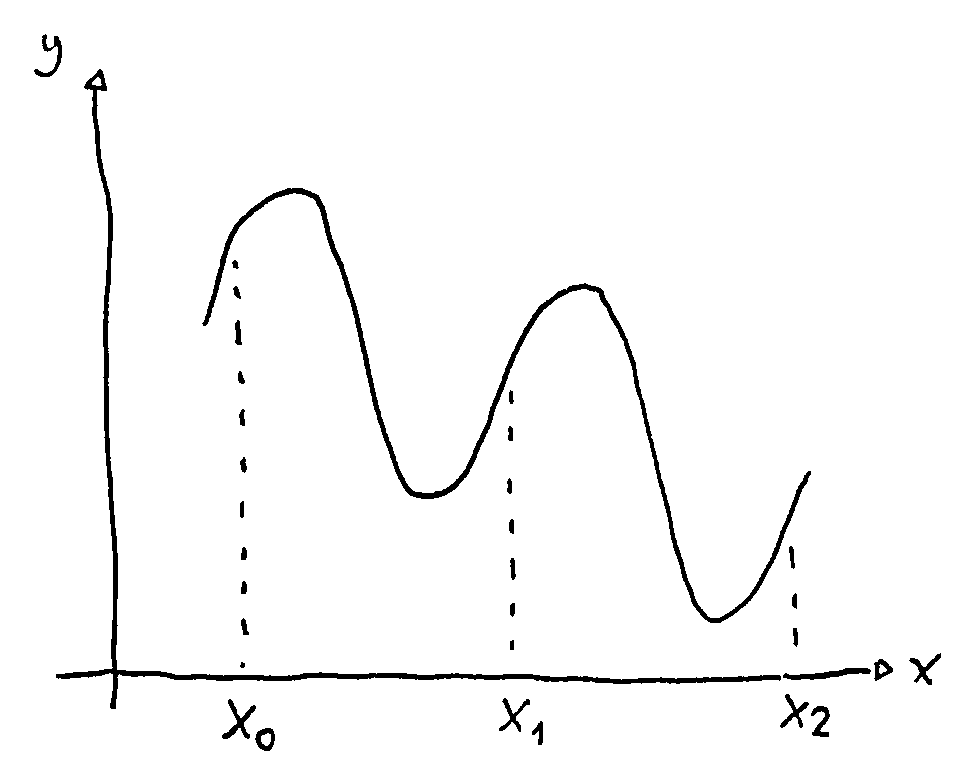
\includegraphics[height=5cm]{2021-2-C2/20211217_infs_e_sups_ex10.pdf}$$


\msk

\newpage

{\bf Exercício 10 (cont.)}

\msk

a) desenhe sobre a primeira delas
%
$$\sup(F([x_0,x_1]))·(x_1-x_0) + \sup(F([x_1,x_2]))·(x_2-x_1),$$ 

b) desenhe sobre a segunda delas
%
$$\inf(F([x_0,x_1]))·(x_1-x_0) + \inf(F([x_1,x_2]))·(x_2-x_1).$$
















  % (mpgp 8 "comprehension")
  % (mpga   "comprehension")


% (c2m212somas2p 23 "exercicio-6")
% (c2m212somas2a    "exercicio-6")
% (c2m212somas2p 24 "exercicio-7")
% (c2m212somas2a    "exercicio-7")
% (c2m212somas2p 25 "exercicio-7-figura")
% (c2m212somas2a    "exercicio-7-figura")
% (c2m212somas2p 26 "dois-jeitos-imagens")
% (c2m212somas2a    "dois-jeitos-imagens")









%\printbibliography

\GenericWarning{Success:}{Success!!!}  % Used by `M-x cv'

\end{document}

%  ____  _             _         
% |  _ \(_)_   ___   _(_)_______ 
% | | | | \ \ / / | | | |_  / _ \
% | |_| | |\ V /| |_| | |/ /  __/
% |____// | \_/  \__,_|_/___\___|
%     |__/                       
%
% «djvuize»  (to ".djvuize")
% (find-LATEXgrep "grep --color -nH --null -e djvuize 2020-1*.tex")

 (eepitch-shell)
 (eepitch-kill)
 (eepitch-shell)
# (find-fline "~/2021.2-C2/")
# (find-fline "~/LATEX/2021-2-C2/")
# (find-fline "~/bin/djvuize")

cd /tmp/
for i in *.jpg; do echo f $(basename $i .jpg); done

f () { rm -v $1.pdf;  textcleaner -f 50 -o  5 $1.jpg $1.png; djvuize $1.pdf; xpdf $1.pdf }
f () { rm -v $1.pdf;  textcleaner -f 50 -o 10 $1.jpg $1.png; djvuize $1.pdf; xpdf $1.pdf }
f () { rm -v $1.pdf;  textcleaner -f 50 -o 20 $1.jpg $1.png; djvuize $1.pdf; xpdf $1.pdf }

f () { rm -fv $1.png $1.pdf; djvuize $1.pdf }
f () { rm -fv $1.png $1.pdf; djvuize WHITEBOARDOPTS="-m 1.0 -f 15" $1.pdf; xpdf $1.pdf }
f () { rm -fv $1.png $1.pdf; djvuize WHITEBOARDOPTS="-m 1.0 -f 30" $1.pdf; xpdf $1.pdf }
f () { rm -fv $1.png $1.pdf; djvuize WHITEBOARDOPTS="-m 1.0 -f 45" $1.pdf; xpdf $1.pdf }
f () { rm -fv $1.png $1.pdf; djvuize WHITEBOARDOPTS="-m 0.5" $1.pdf; xpdf $1.pdf }
f () { rm -fv $1.png $1.pdf; djvuize WHITEBOARDOPTS="-m 0.25" $1.pdf; xpdf $1.pdf }
f () { cp -fv $1.png $1.pdf       ~/2021.2-C2/
       cp -fv        $1.pdf ~/LATEX/2021-2-C2/
       cat <<%%%
% (find-latexscan-links "C2" "$1")
%%%
}

f 20211217_infs_e_sups_ex10



%  __  __       _        
% |  \/  | __ _| | _____ 
% | |\/| |/ _` | |/ / _ \
% | |  | | (_| |   <  __/
% |_|  |_|\__,_|_|\_\___|
%                        
% <make>

 (eepitch-shell)
 (eepitch-kill)
 (eepitch-shell)
# (find-LATEXfile "2019planar-has-1.mk")
make -f 2019.mk STEM=2021-2-C2-infs-e-sups veryclean
make -f 2019.mk STEM=2021-2-C2-infs-e-sups pdf

% Local Variables:
% coding: utf-8-unix
% ee-tla: "c2is"
% ee-tla: "c2m212is"
% End:
